\documentclass{jarticle}
\usepackage[dvipdfmx]{graphicx}
\usepackage{here}
\usepackage{listings,jlisting}
\usepackage{amsmath}

\lstset{
  basicstyle={\ttfamily},
  identifierstyle={\small},
  commentstyle={\smallitshape},
  keywordstyle={\small\bfseries},
  ndkeywordstyle={\small},
  stringstyle={\small\ttfamily},
  frame={tb},
  breaklines=true,
  columns=[l]{fullflexible},
  numbers=left,
  xrightmargin=0zw,
  xleftmargin=3zw,
  numberstyle={\scriptsize},
  stepnumber=1,
  numbersep=1zw,
  lineskip=-0.5ex
}

\title{{システム実験}\\実験後期第1回レポート}
\author{6119019056 山口力也}
\date{2019/10/10日提出}
\begin{document}
\maketitle
\section{課題11.1}
課題11.1で作成したプログラム(Arduino)を報告せよ. \\
以下ソースコード\ref{code:kadai11-1-1-a}に作成したプログラムのソースコードを示す.

\lstinputlisting[caption = 課題11.1.1(Arduino),label=code:kadai11-1-1-a]{arduino/kadai11-1-1/kadai11-1-1.ino}

\section{課題11.2}
課題11.2で作成したプログラムを報告せよ. \\
以下ソースコード\ref{code:kadai11-1-2-a},に\ref{code:kadai11-1-2-p}作成したプログラムのソースコードを示す.

\lstinputlisting[caption = 課題11.1.2(Arduino),label=code:kadai11-1-2-a]{arduino/kadai11-1-2/kadai11-1-2.ino}
\lstinputlisting[caption = 課題11.1.2(Processing),label=code:kadai11-1-2-p]{processing/kadai11_1_2/kadai11_1_2.pde}

また、結果の画像を以下\ref{fig:kadai11-1-2}に示す.
\begin{figure}[H]
\begin{center}
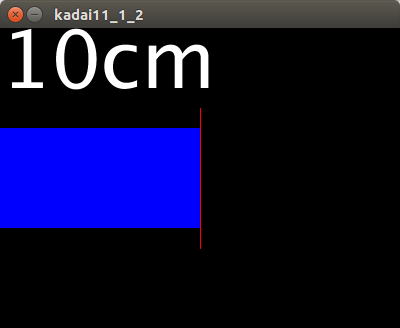
\includegraphics[width=7.0cm]{figures/kadai11-1-2.png}
\caption{課題11.1.2の結果}
\label{fig:kadai11-1-2}
\end{center}
\end{figure}

\section{発展課題11.3}
発展課題11.3で作成したプログラムを報告せよ. \\
図形を描くようにロボットを移動させるには,任意の角度だけ回転させる必要がある.これをどのように実現したか,そのアルゴリズムを解説せよ.

以下ソースコード\ref{code:kadai11-1-1-a}に作成したプログラムのソースコードを示す.

\lstinputlisting[caption = 発展課題11.1.3(Arduino),label=code:kadai11-1-3-a]{arduino/hattenkadai11-1-3/hattenkadai11-1-3.ino}

任意の角度を回転させるには経験的に何秒ほどdelayをいれることでどれだけ回転するかを測って行なった.


\end{document}




